% File: datasheet.tex
% Author: Y.U.P. (yashparitkar)
% Last Modified: 2026-08-13 Thu 19:47
%
% Description: LaTeX source file for the LibreILA datasheet. This covers the technical specifications and features of the LibreILA tool.

\documentclass[twocolumn]{article}
\usepackage{float}
\usepackage{stfloats}   % allows full-width (figure*/table*) floats at the bottom of a page too
\usepackage[margin=2.5cm]{geometry}
\setlength{\columnsep}{0.8cm}   % gutter between the two columns
% \usepackage{xurl}
\usepackage{tabularx}
\usepackage{multicol}   % two-column table of contents on an otherwise one-column page
\usepackage[utf8x]{inputenc}
\usepackage{amssymb}
\usepackage{amsmath}
\usepackage{tikz}
\usepackage{xcolor}
\usepackage{colortbl}
\usepackage[linktocpage]{hyperref}
% \usepackage{wasysym}
\usepackage{graphicx}
% \usepackage{epsfig}
% Default graphic width. Use \linewidth (NOT \textwidth): inside a normal
% `figure` \linewidth is the column width, inside a `figure*` it is the full
% page width, so the same default works in both cases.
\setkeys{Gin}{width=0.8\linewidth}
% \usepackage[normalem]{ulem}
% \usepackage{enumerate}
\usepackage{listings}
\usepackage[nohyperlinks,nolist]{acronym}
\usepackage{enumitem}
\usepackage{hhline}   % rules that survive a coloured cell, see the regdiag block

% Hex literal. \ensuremath so the same macro works in prose and inside a
% math expression like the sample buffer offset; \mathtt so the x stays
% upright instead of being set as a maths variable.
\newcommand{\hex}[1]{\ensuremath{\mathtt{0x#1}}}

%% List spacing %%%%%%%%%%%%%%%%%%%%%%%%%%%%%%%%%%%%%%%%%%%%%%%%%%%%%%
% The default list glue is elastic (\itemsep is 4pt plus 2pt minus 1pt,
% \topsep and \parsep likewise), and article.cls turns on \flushbottom
% for a twocolumn document and never turns it off again -- not even
% under the \onecolumn used for the body. Every page therefore gets
% padded out to the full column height, and since a list is usually the
% only stretchable glue on the page, the whole shortfall lands between
% the items. That is why the same itemize looks tight on one page and
% loose on the next.
%
% Fix both halves: rigid spacing so a list cannot be stretched, and
% \raggedbottom so LaTeX stops trying to. Pages now end where their
% content ends.
\setlist{topsep=4pt, itemsep=2pt, parsep=0pt, partopsep=0pt}
\raggedbottom


\lstset{ %
basicstyle=\footnotesize,       % the size of the fonts that are used for the code
showspaces=false,               % show spaces adding particular underscores
showstringspaces=false,         % underline spaces within strings
showtabs=false,                 % show tabs within strings adding particular underscores
frame=single,                   % adds a frame around the code
tabsize=2,                      % sets default tabsize to 2 spaces
breaklines=true,                % sets automatic line breaking
breakatwhitespace=false,        % sets if automatic breaks should only happen at whitespace
}

\hypersetup{
 colorlinks=true,
 citecolor=violet,
 linkcolor=blue,
 urlcolor=blue
}

\usepackage{fancyhdr}


\usepackage{subfiles} % Allows compiling individual chapters/appendices standalone; load last


\fancyhead[L]{LibreILA Datasheet}
\fancyhead[R]{Yash Paritkar}
\fancyfoot[L]{\leftmark}
\fancyfoot[C]{}
\fancyfoot[R]{\thepage}
\renewcommand{\headrulewidth}{0.5pt}
\renewcommand{\footrulewidth}{0.5pt}
\pagestyle{fancy}


\newcommand{\todo}[1]{\textbf{\color{red}TODO: #1}}
\newcommand{\arya}{\color{blue}}
\newcommand{\degr}{\ensuremath{^\circ}}

%% Register bit-field diagrams %%%%%%%%%%%%%%%%%%%%%%%%%%%%%%%%%%%%%%%
% One `regdiag` is one row of eight bits in the style of the Microchip
% core user guides: a row of bit numbers, a boxed row of fields, then
% the access and reset of each bit. Four of them make a 32-bit register.
%
%   \begin{regdiag}
%     \bitnums{7}{6}{5}{4}{3}{2}{1}{0}
%     \fldrow{\rsvdb{5}\fld{3}{FOO[2:0]}}
%     \bitacc{}{}{}{}{}{R}{R}{R}
%     \bitrst{}{}{}{}{}{0}{0}{0}
%   \end{regdiag}
%
% The column spec carries no rules at all. The verticals come from the
% \multicolumn in the field row and the horizontals from \bitrule, so
% only that row is boxed and the other three stay clean. \fldb starts a
% field row because it is the one that has to draw the left edge, \fld
% continues it; \rsvdb/\rsvdc are their greyed reserved counterparts.
%
% \bitrule is \hhline rather than the obvious \cline{2-9}. colortbl's
% coloured panel is painted after the rules and overhangs the row by one
% \arrayrulewidth at the top, so a \cline above a greyed cell is drawn
% and then covered up -- which is why the reserved rows came out with no
% top edge. \hhline puts its rule just clear of the panel instead, and
% spans exactly the same width, so only the greyed rows change.
% Nine equal columns filling \textwidth: the Bit/Access/Reset label gets
% the same width as one bit, so 1 + 8 spans margin to margin. \tabcolsep
% is 2pt and the outer pair is killed by @{}, leaving eight inter-column
% gaps of 2*\tabcolsep = 32pt to take off the total. The extra 1pt is
% slack for the field row's outer vertical rules, which add
% 2*\arrayrulewidth on top of the column widths and would otherwise tip
% the row over the right margin.
% \regcolw is worked out inside the environment rather than here, so it
% picks up whatever \textwidth geometry has settled on.
\newlength{\regcolw}

\newcolumntype{Y}{>{\centering\arraybackslash}p{\regcolw}}
% The label column is as wide as a bit column but keeps its text against
% the diagram, as in the reference guides.
\newcolumntype{L}{>{\raggedleft\arraybackslash}p{\regcolw}}

% Ragged-right X for the wide tabularx tables. Justifying a narrow X column
% leaves large interword gaps and a stream of underfull-hbox warnings.
\newcolumntype{P}{>{\raggedright\arraybackslash}X}

\newenvironment{regdiag}{%
  \par\nobreak\vspace{0.5em}%
  \footnotesize
  \renewcommand{\arraystretch}{1.25}%
  \setlength{\tabcolsep}{2pt}%
  \setlength{\regcolw}{\dimexpr(\textwidth - 33pt)/9\relax}%
  \noindent\begin{tabular}{@{}L*{8}{Y}@{}}%
}{%
  \end{tabular}\par\vspace{0.4em}%
}

\newcommand{\bitrule}{\hhline{~*{8}{-}}}
\newcommand{\bitnums}[8]{Bit & #1 & #2 & #3 & #4 & #5 & #6 & #7 & #8 \\ \bitrule}
\newcommand{\fldrow}[1]{ & #1 \\ \bitrule}
\newcommand{\bitacc}[8]{Access & #1 & #2 & #3 & #4 & #5 & #6 & #7 & #8 \\}
\newcommand{\bitrst}[8]{Reset & #1 & #2 & #3 & #4 & #5 & #6 & #7 & #8 \\}

% The continuation forms carry the & themselves, so a field row reads as
% one run of fields with no separators to get wrong.
\newcommand{\fldb}[2]{\multicolumn{#1}{|c|}{#2}}          % first field of a row
\newcommand{\fld}[2]{& \multicolumn{#1}{c|}{#2}}          % any later field
\newcommand{\rsvdb}[1]{\multicolumn{#1}{|c|}{\cellcolor{gray!25}}}
\newcommand{\rsvdc}[1]{& \multicolumn{#1}{c|}{\cellcolor{gray!25}}}
\newcommand{\rsvdrow}{\fldrow{\rsvdb{8}}}                 % a wholly reserved byte
\newcommand{\emptyrow}{\bitacc{}{}{}{}{}{}{}{}\bitrst{}{}{}{}{}{}{}{}}

% The property block that heads every register subsection
\newcommand{\regprop}[5]{%
  \begin{tabular}{ll}
    \textbf{Name:}         & #1 \\
    \textbf{Register Set:} & #2 \\
    \textbf{Offset:}       & #3 \\
    \textbf{Reset:}        & #4 \\
    \textbf{Property:}     & #5 \\
  \end{tabular}\par\vspace{0.6em}%
}

\title{LibreILA Datasheet}
\author{Yash Paritkar (github/yashparitkar)}
\date{August 2026}

\begin{document}
%% Acronym definitions. These have to come before the first \acs, and the
%% `nolist' option means the environment itself prints nothing, so it can
%% sit here at the very top of the body.
\begin{acronym}[sort = true]
    % A
    \acro{AXI}{Advanced eXtensible Interface}
    % C
    \acro{CDC}{Clock Domain Crossing}
    % F
    \acro{FIFO}{First In First Out (queue)}
    \acro{FPGA}{Field Programmable Gate Array}
    % G
    \acro{GUI}{Graphical User Interface}
    % H
    \acro{HDL}{Hardware Description Language}
    % I
    \acro{ILA}{Integrated Logic Analyzer}
    \acro{IP}{Intellectual Property}
    % L
    \acro{LSRAM}{Large Static Random Access Memory}
    % O
    \acro{OHL}{Open Hardware Licence}
    % R
    \acro{RTL}{Register Transfer Level}
    % S
    \acro{SDC}{Synopsys Design Constraints}
    % U
    \acro{UART}{Universal Asynchronous Receiver Transmitter}
    % V
    \acro{VCD}{Value Change Dump}
\end{acronym}

%% Front matter: full page width, no columns %%%%%%%%%%%%%%%%%%%%%%%%
\onecolumn

%% Title page %%%%%%%%%%%%%%%%%%%%%%%%%%%%%%%%%%%%%%%%%%%%%%%%%%%%%%%
\thispagestyle{plain}
\twocolumn
\begin{table*}
    % Tightened from the default 6pt: at 6pt the title row is a few points
    % wider than \textwidth and the row overfulls.
    \setlength{\tabcolsep}{3pt}
    \begin{tabular}{cc}
        {
            \raisebox{-0.5\height}{\includegraphics[width = 3cm]{./images/libre_ila_logo_converted.pdf}}
        } &
        {
            \begin{tabular}[c]{l}
                \textbf{\Large LibreILA (Integrated Logic Analyzer) Datasheet} \\
                \textbf{Version: 0.2} \\
                \textbf{Date: August 2026} \\
                \textbf{Author: Yash Paritkar (github/yashparitkar)} \\
                \textbf{License: CERN \acs{OHL} v2 -- Permissive} \\
            \end{tabular}
        }
    \end{tabular}
\end{table*}

\section{Features}
\begin{itemize}
    \item Open-source and free to use: \\ \url{github.com/yashparitkar/libreila}
    \item Probe of any width, described by a CSV file. The same bit order is shared by the trigger vector, the sample buffer and both host drivers
    \item Pass-through probe splice, combinational, adding no latency to the probed link
    \item Capture into fabric RAM, one sample per sampling clock edge while armed, read back over AXI4Lite
    \item Customizable trigger:
    \begin{itemize}
        \item Condition and mask, one bit per probed bit, reduced by AND or by OR
        \item Level, rising edge or falling edge
        \item Adjustable trigger position within the captured window
        \item Force trigger and disarm from the host, so a condition that never occurs costs a register write rather than a reset
        \item Optional external trigger input, selected at synthesis
        \item Trigger output for chaining several instances onto one event
    \end{itemize}
    \item Two independent clock domains, with the arm, disarm and status paths synchronised
    \item Per-instance identity register, so a system holding several cores can tell them apart
    \item A serial wrapper is also provided to easily use the \acs{ILA} with PC, needing no processor and no vendor debug tooling in the design
    \item A python driver is provided to configure the \acs{ILA} over the serial wrapper and dump the capture as a \acs{VCD} for any waveform viewer, with command line and \acs{GUI} front ends. A baremetal C driver is provided for the bare AXI4Lite core
    \item Plain VHDL-2008 throughout, with no vendor primitives instantiated
    \item A default example is provided to use the \acs{ILA} with a simple 64-bit AXI4Stream interface
\end{itemize}

\section{Application}
\begin{itemize}
    \item RTL debugging
    \item FPGA prototyping
    \item Generic logic analyser
\end{itemize}

\section{Description}
LibreILA is an in-system \acf{ILA} for \acs{FPGA} designs, written in plain VHDL. It is spliced into a link inside the fabric and samples it into a circular buffer held in fabric RAM, so nets that never reach a pad are as visible as the ones that do. The host sets a condition on the probed bits, arms the core, and reads back a window of samples from either side of the point at which that condition occurred.

The core observes one flat probe word of \texttt{G\_PROBE\_WIDTH} bits and attaches no meaning to it. That bit order is shared by the trigger, the sample buffer and both drivers, and a build is described entirely by two CSV files.

Two deliverables are provided. \texttt{libre\_ila} is the core itself, with an AXI4Lite slave port and a baremetal C driver, for a design that already carries a bus master. \texttt{libre\_ila\_uart} wraps it with a \acs{UART} and a packet parser and is driven from a PC over two wires by the python driver. Neither needs vendor debug tooling in the design.

\begin{table}[H]
    \centering
    \footnotesize
    \begin{tabularx}{\linewidth}{|l|P|}
        \hline
        \rowcolor{gray!40} \textbf{Parameter} & \textbf{Specification} \\
        \hline
        Probe width    & Any width of one bit or more, set at synthesis \\
        \hline
        Buffer depth   & Power of two, two samples or more \\
        \hline
        Sampling       & One sample per \texttt{samp\_aclk} edge while armed \\
        \hline
        Storage        & \texttt{DEPTH} $\times \lceil$\texttt{WIDTH}$/32\rceil \times 32$ bits of fabric RAM \\
        \hline
        Probe latency  & None, the splice is combinational \\
        \hline
        Max \texttt{samp\_aclk} & 243 MHz, stock build, PolarFire SoC \\
        \hline
        Host interface & AXI4Lite slave, or \acs{UART} 8N1 on the wrapper \\
        \hline
        Language       & VHDL-2008, no vendor primitives \\
        \hline
    \end{tabularx}
    \caption{Key specifications}
    \label{tab:keyspec}
\end{table}

\newpage
\onecolumn
\begin{multicols}{2}
\tableofcontents
\end{multicols}

\section{Revision History}

\renewcommand{\arraystretch}{1.5}
\begin{table}[H]
    \centering
    \begin{tabularx}{\textwidth}{|l|c|P|}
        \hline
        \rowcolor{gray!40} \textbf{Version} & \textbf{Date} & \textbf{Comments} \\
        \hline
        0.0 & 25 July 2026 & Document created.\\
        \hline
        0.1 & 4 August 2026 & DISARM mapped onto the reserved input register at \hex{2C}.\\
        \hline
        0.2 & 13 August 2026 & Added the capture procedure, reset, timing characteristics, timing constraints and device requirements sections. Corrected the external trigger description: \texttt{i\_ext\_trig} is edge detected but not synchronised inside the core.\\
        \hline
        \end{tabularx}
    \caption{Revision history}
    \label{tab:history}
\end{table}
\renewcommand{\arraystretch}{1.0}

%% Body: back to one column %%%%%%%%%%%%%%%%%%%%%%%%%%%%%%%%%%%%%%%%%
\newpage
\section{Detailed description}
This section says how it works: what the blocks are, how a capture proceeds from arming to readout, and where the two clock domains meet. The register-level detail that a driver needs is in Section~\ref{sec:regsummary}.

\subsection{Overview}
Everything in the core is arranged around one shared definition of the probe word, \texttt{w\_probe}. Three blocks sit on top of it:

\begin{itemize}
    \item \textbf{The probe splice.} A pair of mirrored ports shorted combinationally, so the probed link passes straight through and the core reads it in parallel.
    \item \textbf{The trigger comparator.} One condition bit and one mask bit per probed bit, reduced to a single condition and then qualified by the level or edge mode.
    \item \textbf{The sample buffer and the AXI4Lite slave.} A circular buffer in fabric RAM, written every sampling clock while armed and read back as a flat register map.
\end{itemize}

A capture runs in one direction. The host writes the trigger condition, the mask, the mode and the trigger position, then writes ARM\_FT. The core starts sampling into the buffer immediately, overwriting the oldest sample once it wraps, so that at any moment the buffer holds the most recent \texttt{G\_SAMP\_BUFF\_DEPTH} samples. When the trigger condition is met the core latches where it happened, keeps sampling for the configured number of post-trigger samples, and stops. DONE then goes high and the buffer holds a window of history either side of the trigger. Sampling has stopped by that point, so the host may read the buffer back at any rate it likes without disturbing the capture. A capture still in progress can be cancelled at any point by writing DISARM, which returns the core to IDLE from either side of the trigger; a capture already finished is left alone.

\begin{figure}[H]
    \centering
    \includegraphics[width=0.8\textwidth]{images/architecture_diagram_core_fabric.drawio_converted.pdf}
    \caption{LibreILA core block diagram}
    \label{fig:libre_ila_core_bd}
\end{figure}

The core straddles two clock domains and is deliberate about which side each part lives on. Sampling, triggering and the buffer write port run on \texttt{samp\_aclk}, the clock of the probed link. The register map and the buffer read port run on \texttt{S\_AXIL\_ACLK}. Only the arm and disarm pulses and the three status bits actually cross, through two-flop synchronisers; the sample data never crosses a synchroniser at all, because the buffer is a dual-port RAM whose read port is simply clocked from the other domain.

\begin{figure}[H]
    \centering
    \includegraphics[width=0.8\textwidth]{images/architecture_diagram_liu_fabric.drawio_converted.pdf}
    \caption{LibreILA UART block diagram}
    \label{fig:libre_ila_uart_bd}
\end{figure}

\texttt{libre\_ila\_uart} wraps all of the above with a \acs{UART} and a packet parser, putting the same register map at the end of a serial link instead of on an AXI bus. Nothing inside the core changes.

\subsection{The probe}
The core samples one vector, \texttt{w\_probe}, of \texttt{G\_PROBE\_WIDTH} bits. Signals are packed LSB first in the order they are listed in \texttt{portmap.csv}, and that concatenation is the single definition of the probe bit order: the sample buffer, the trigger vector and both drivers inherit it. For the stock 64-bit AXI4Stream build the probe is 67 bits wide, laid out as in Table~\ref{tab:stockprobe}.

\begin{table}[H]
    \centering
    \begin{tabular}{|l|l|}
        \hline
        \rowcolor{gray!40} \textbf{Bit range} & \textbf{Signal} \\
        \hline
        63 downto 0 & TDATA \\
        \hline
        64 & TLAST \\
        \hline
        65 & TVALID \\
        \hline
        66 & TREADY \\
        \hline
    \end{tabular}
    \caption{Probe word of the stock AXI4Stream build}
    \label{tab:stockprobe}
\end{table}

The core is spliced into the link it probes, so the probe appears as a pair of mirrored ports named after the role the core plays on each side, not after the direction the data happens to flow:

\begin{itemize}
    \item \texttt{probe\_slave\_*} faces the \emph{master} of the probed link, so the core is the slave there, and these ports carry the directions listed in \texttt{portmap.csv}.
    \item \texttt{probe\_master\_*} faces the \emph{slave} of the probed link, so the core is the master there, and every direction is the mirror of its \texttt{probe\_slave\_} twin.
\end{itemize}

The two sides are shorted combinationally, so the splice is purely pass through and introduces no delay into the probed link. A signal that cannot be spliced in series is tapped in parallel instead, with the \texttt{mon} type, which the core reads and never drives.

\subsection{Capture}
While the \acs{ILA} is armed it stores one sample of the probe word per rising edge of \texttt{samp\_aclk} into a circular buffer \texttt{G\_SAMP\_BUFF\_DEPTH} samples deep. Once the trigger fires the core keeps capturing for \texttt{DEPTH - TRIG\_POS - 1}  further samples and then stops, so the captured window holds \texttt{TRIG\_POS} samples of history ahead of the trigger and the rest behind it.

Because the buffer is circular, the oldest sample is not at index zero and the window is almost always split across the wrap point. The core reports where the window starts and where the trigger landed in SAMP\_BUFF\_FRST\_IDX and SAMP\_BUFF\_TRIG\_IDX, and the host unrolls the buffer from there. Figure~\ref{fig:sampbuff} shows the two views: the capture as it happened, and the same samples as they sit in the buffer.

\begin{figure}[H]
    \centering

    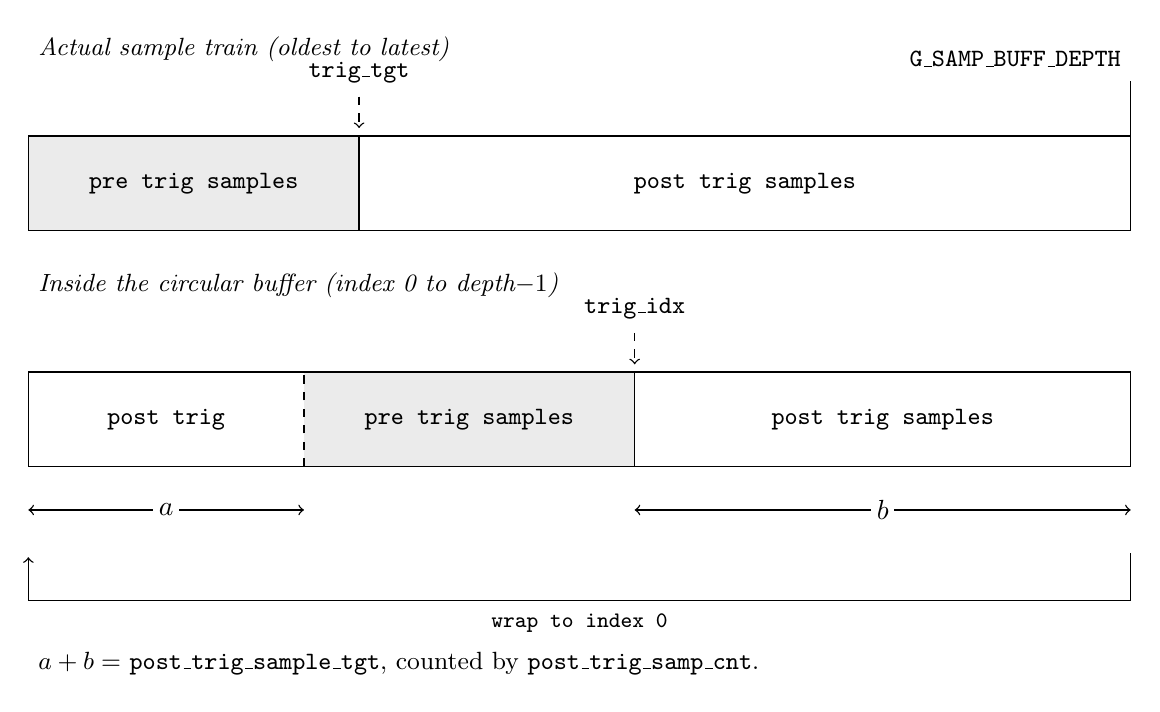
\begin{tikzpicture}[x=1cm,y=1cm,line width=0.5pt]

        % ------------------------------------------------ band 1: sample train
        \node[anchor=west,font=\itshape\small] at (0,2.3) {Actual sample train (oldest to latest)};

        \fill[black!8] (0,0) rectangle (4.2,1.2);
        \draw (0,0) rectangle (14,1.2);
        \draw (4.2,0) -- (4.2,1.2);
        \node[font=\ttfamily\small] at (2.1,0.6)  {pre trig samples};
        \node[font=\ttfamily\small] at (9.1,0.6)  {post trig samples};

        \draw[dashed,->] (4.2,1.7) -- (4.2,1.3);
        \node[font=\ttfamily\small,anchor=south] at (4.2,1.75) {trig\_tgt};
        \draw (14,1.2) -- (14,1.9);
        \node[font=\ttfamily\small,anchor=south east] at (14,1.95) {G\_SAMP\_BUFF\_DEPTH};

        % ------------------------------------------------ band 2: circular buffer
        \begin{scope}[yshift=-3cm]
        \node[anchor=west,font=\itshape\small] at (0,2.3) {Inside the circular buffer (index 0 to depth$-1$)};

        \fill[black!8] (3.5,0) rectangle (7.7,1.2);
        \draw (0,0) rectangle (14,1.2);
        \draw[dashed] (3.5,0) -- (3.5,1.2);
        \draw (7.7,0) -- (7.7,1.2);
        \node[font=\ttfamily\small] at (1.75,0.6)  {post trig};
        \node[font=\ttfamily\small] at (5.6,0.6)   {pre trig samples};
        \node[font=\ttfamily\small] at (10.85,0.6) {post trig samples};

        \draw[dashed,->] (7.7,1.7) -- (7.7,1.3);
        \node[font=\ttfamily\small,anchor=south] at (7.7,1.75) {trig\_idx};

        % a / b spans
        \draw[<->] (0,-0.55)   -- (3.5,-0.55);
        \draw[<->] (7.7,-0.55) -- (14,-0.55);
        \node[fill=white,inner sep=2pt] at (1.75,-0.55)  {$a$};
        \node[fill=white,inner sep=2pt] at (10.85,-0.55) {$b$};

        % wrap: leaves the right edge, re-enters at index 0
        \draw[->] (14,-1.1) -- (14,-1.7) -- (0,-1.7) -- (0,-1.15);
        \node[font=\ttfamily\footnotesize,anchor=north] at (7,-1.75) {wrap to index 0};
        \end{scope}

        \node[anchor=west,font=\small] at (0,-5.5)
        {$a + b =$ \texttt{post\_trig\_sample\_tgt}, counted by \texttt{post\_trig\_samp\_cnt}.};

        \end{tikzpicture}

    \caption{The sample buffer is a circular buffer. The capture starts once the \acs{ILA} is armed, and the trigger can happen anywhere in the buffer. The host can unroll the buffer in software from the reported start index and trigger index.}
    \label{fig:sampbuff}
\end{figure}

That split is also what the post-trigger counter inside the core counts out: it targets $a + b$ samples, not the distance to the end of the buffer.

\subsection{Trigger}
The trigger is one condition bit per probed bit, held in two registers of identical layout. TRIG\_COND carries the value each probe bit has to take to match, TRIG\_MASK decides whether that bit takes part at all. The enabled bits are then reduced to a single condition, by AND or by OR, and that single condition is what the level and edge modes act on (Table~\ref{tab:trigmodes}).

\begin{table}[H]
    \centering
    \begin{tabular}{|c|c|l|l|}
        \hline
        \rowcolor{gray!40} \textbf{EDGE} & \textbf{FALLING} & \textbf{Mode} & \textbf{Triggers when the condition} \\
        \hline
        0 & x & Level   & \emph{is} true \\
        \hline
        1 & 0 & Rising  & \emph{becomes} true \\
        \hline
        1 & 1 & Falling & \emph{becomes} false \\
        \hline
    \end{tabular}
    \caption{Trigger modes, \texttt{TRIG\_CFG} bits 2 and 1}
    \label{tab:trigmodes}
\end{table}

The distinction matters at arming time. In level mode a condition that already holds when the \acs{ILA} is armed fires on the very first sample and captures nothing of interest, as ``trigger when TVALID is high'' would on a mostly idle stream. The edge modes wait for a transition instead, and a condition that is already true at the moment of arming is not mistaken for a rising edge.

Edge detection is applied to the reduced condition and not per probe bit. Asking for ``bit 5 rises \emph{and} bit 9 falls in the same sample'' is therefore not expressible.

Note that an all-zero TRIG\_MASK in AND mode matches vacuously and fires on the first sample after arming. Use OR mode with an all-zero mask if the intent is never to trigger on the probe.

\subsection{External trigger and chaining}
Setting \texttt{G\_EXTERNAL\_TRIG} to 1 replaces the trigger comparator with the \texttt{i\_ext\_trig} pin: in that build the \acs{ILA} triggers only on the rising edge of that pin, and the three TRIG\_CFG mode bits, TRIG\_COND and TRIG\_MASK are all ignored. The trigger vector logic is not synthesised at all, which is why the external trigger build is the smaller of the two in Table~\ref{tab:utilization-core}.

The edge is detected by a single flop in the sampling domain and \texttt{i\_ext\_trig} is \textbf{not} synchronised inside the core. It must therefore be driven from logic already running on \texttt{samp\_aclk}, or synchronised externally before it reaches the pin.

The resulting trigger is driven out on \texttt{o\_trig\_out} in every build, so several instances can be chained to capture one event across different parts of a design: \texttt{o\_trig\_out} of one instance drives \texttt{i\_ext\_trig} of the next. Chained instances must share a sampling clock, or carry a synchroniser between them, for the same reason.

\subsection{Clock domains}
The capture side runs entirely in the sampling clock domain, driven by \texttt{samp\_aclk}, which should be fed the clock the probed link runs on. The AXI4Lite port is a separate domain on \texttt{s\_axil\_aclk}. The arm and disarm pulses and the ARMED, TRIGD and DONE status bits cross between them through two-flop synchronisers and so lag by a couple of cycles; the internal STATE field of the status register is not synchronised and is there for debugging only.

Arm and disarm cross on separate paths, each a write-toggled bit resynchronised and edge-detected on the sampling side. Two writes close together can therefore land in either order in the sampling domain. A host that writes both back to back should leave at least five sampling clock periods between them if it cares which one wins.

Readout needs no synchroniser at all. The sample buffer is a simple dual-port RAM whose write port is clocked by \texttt{samp\_aclk} and whose read port is clocked by \texttt{s\_axil\_aclk}, so the sample data never crosses a synchroniser and never needs to.

\subsection{Readout}
Samples are stored one 32-bit lane per slice of the probe word, so lane $n$ carries probe bits $32n+31$ downto $32n$ and the last lane is zero padded in its upper bits. On readout the lanes are padded further, up to \texttt{C\_AXIL\_STRIDE} registers per sample. The trigger vector uses that same padded layout, so a captured sample and a trigger condition are directly comparable word for word, and a sample read back can be written straight into TRIG\_COND to trigger on its recurrence.

\subsection{Reset}
The core takes two resets, one per clock domain. \texttt{i\_rst\_sync} is active high and is sampled in the sampling clock domain; it clears the capture state machine, the write pointer and the trigger index. \texttt{s\_axil\_aresetn} is active low and is sampled in the AXI4Lite domain; it clears the register map and the AXI4Lite state machines. The sample buffer contents are not cleared by either, since a capture always overwrites the whole buffer before it can complete.

Both resets must be held for at least two periods of the clock that samples them. \texttt{libre\_ila\_uart} drives \texttt{s\_axil\_aresetn} internally from \texttt{i\_rst\_sync}, so the wrapper takes a single reset input; hold it for at least two periods of the \emph{slower} of the two clocks.

\subsection{Timing characteristics}
The figures in Table~\ref{tab:timing} are cycle counts through the core's own logic and hold for any build. The one cycle of uncertainty on the arm and disarm paths is the resolution time of the first synchroniser flop.

\begin{table}[H]
    \centering
    \begin{tabularx}{\textwidth}{|P|l|}
        \hline
        \rowcolor{gray!40} \textbf{Parameter} & \textbf{Value} \\
        \hline
        Probe input to probe output, through the splice & Combinational, 0 \\
        \hline
        ARM\_FT write accepted to first sample stored & 4 to 5 \texttt{samp\_aclk} \\
        \hline
        DISARM write accepted to IDLE & 4 to 5 \texttt{samp\_aclk} \\
        \hline
        Trigger condition true to the sample recorded at SAMP\_BUFF\_TRIG\_IDX & 0, it is that sample \\
        \hline
        Trigger to DONE & \texttt{DEPTH}$-$\texttt{TRIG\_POS}$-1$ \texttt{samp\_aclk} \\
        \hline
        Capture state change to ARMED, TRIGD or DONE readable over AXI4Lite & 2 \texttt{s\_axil\_aclk} \\
        \hline
        Minimum spacing between an ARM\_FT and a DISARM write for the order to be guaranteed & 5 \texttt{samp\_aclk} \\
        \hline
    \end{tabularx}
    \caption{Timing characteristics}
    \label{tab:timing}
\end{table}

The trigger index is exact: the sample stored at SAMP\_BUFF\_TRIG\_IDX is the one on which the condition held, in level mode, or the one on which it changed, in the edge modes. No correction for pipeline delay is needed on the host side.

Readout time over the \acs{UART} wrapper follows from the packet format of Section~\ref{sec:uartpkt}. A capture of \texttt{DEPTH} samples is $a \times$\texttt{DEPTH} words, sent in packets of at most 127 words, each carrying a six byte header in both directions. For the stock build that is 8192 words in 65 packets, about 33.5 kB, which at 115\,200 baud 8N1 takes roughly 2.9 seconds.

\subsection{Timing constraints}
\texttt{samp\_aclk} and \texttt{s\_axil\_aclk} are unrelated. Declare them as asynchronous to one another in the constraint file so that the tool does not attempt to close timing between the domains; in \acs{SDC} that is \texttt{set\_clock\_groups -asynchronous}. The paths that genuinely cross are the arm and disarm toggles and the three status bits, all of which carry their own two-flop synchronisers, and the sample buffer, which crosses inside the RAM and needs no constraint.

Where the two clocks are driven from the same source, or where the design constrains them together for other reasons, a maximum delay on the crossing registers is the narrower alternative.

\subsection{Device requirements}
\label{sec:portability}
The core is plain VHDL-2008 and uses only \texttt{ieee.std\_logic\_1164}, \texttt{ieee.numeric\_std} and \texttt{ieee.math\_real}. No vendor primitive is instantiated anywhere, and no vendor library is referenced, so the sources compile as they stand under any VHDL-2008 tool. They are simulated with GHDL in the supplied test suite.

The one thing the core asks of a device is that its synthesis tool infer a \textbf{simple dual-port RAM with independent read and write clocks} from the sample buffer, which is written on \texttt{samp\_aclk} and read on \texttt{s\_axil\_aclk}. Every current FPGA family has such a block. Where a tool declines to infer it the design still builds and still behaves correctly, but the buffer falls back to registers and the resource cost rises sharply, so it is worth checking the synthesis report on a new family.

The buffer carries a \texttt{syn\_ramstyle} attribute of \texttt{"lsram"}, which Synplify and Libero honour and other tools ignore. It is the only vendor-specific text in the sources and changing or removing it does not affect behaviour.

The figures quoted throughout this document were measured on a PolarFire SoC (MPFS Discovery Kit).

\newpage
\section{Capture procedure}
\label{sec:capture}
A capture is a short sequence of register accesses followed by a bulk read. The steps below give the general form; the offsets quoted are those of the stock build, where the stride $a$ is 4. Table~\ref{tab:regsummary} gives the offsets symbolically for any build.

\begin{enumerate}
    \item \textbf{Confirm the core.} Read MGCKEY at \hex{04} and check that it reads \hex{B01DFACE}. Read UID at \hex{14} if the system holds more than one \acs{ILA}.
    \item \textbf{Read the geometry.} WIDTH at \hex{0C} and DEPTH at \hex{10} give the probe width and the buffer depth, from which \texttt{C\_N\_LANES} and the stride $a$ follow. SAMP\_CLK\_FREQ at \hex{08} gives the time axis. Every remaining offset is derived from these, so nothing needs to be known about the build in advance.
    \item \textbf{Set the trigger position.} Write TRIG\_POS at \hex{20} with the number of samples of history to keep before the trigger. The core will capture \texttt{DEPTH}$-$\texttt{TRIG\_POS}$-1$ samples after it.
    \item \textbf{Set the condition.} Write TRIG\_COND$(0 \ldots a-1)$ with the value each probe bit must take, and TRIG\_MASK$(0 \ldots a-1)$ with a 1 for each bit that takes part. Bits left masked off are don't cares.
    \item \textbf{Set the mode.} Write TRIG\_CFG at \hex{28} to select AND or OR reduction and level, rising or falling sensitivity.
    \item \textbf{Arm.} Write any value to ARM\_FT at \hex{24}. Sampling begins within five sampling clocks.
    \item \textbf{Wait.} Poll STATUS at \hex{00} until DONE, bit 2, is set. A second write to ARM\_FT forces the trigger if the condition turns out never to occur; a write to DISARM at \hex{2C} cancels the capture and returns the core to IDLE.
    \item \textbf{Locate the window.} Read SAMP\_BUFF\_FRST\_IDX at \hex{1C} and SAMP\_BUFF\_TRIG\_IDX at \hex{18}. Both are valid once DONE is set.
    \item \textbf{Read the buffer.} Read $a \times$\texttt{DEPTH} words from \hex{50}. Sample $k$, lane $l$ sits at $\hex{50} + 4(ak + l)$.
    \item \textbf{Unroll.} Sample $i$ of the window, counting from the oldest, is at buffer index $(\mathrm{FRST\_IDX} + i) \bmod \mathtt{DEPTH}$. The trigger sample sits at position $(\mathrm{TRIG\_IDX} - \mathrm{FRST\_IDX}) \bmod \mathtt{DEPTH}$ within the unrolled window.
\end{enumerate}

Both supplied drivers carry out this sequence. The python driver additionally unrolls the buffer, applies the signal names from \texttt{portmap.csv} and writes the result as a \acs{VCD} file.

\subsection{Worked example}
Using the stock 64-bit AXI4Stream build of Table~\ref{tab:stockprobe}, capture the start of a packet: trigger when TVALID and TLAST are both high, on the rising edge of that condition, keeping 512 samples of history.

TLAST is probe bit 64 and TVALID is probe bit 65, so both fall in trigger word 2, which carries probe bits 95 downto 64, at bit positions 0 and 1 respectively. TDATA and TREADY take no part and their mask bits stay at zero, as do the padding bits above the probe width. Table~\ref{tab:example} gives the resulting writes.

\begin{table}[H]
    \centering
    \begin{tabularx}{\textwidth}{|l|l|l|P|}
        \hline
        \rowcolor{gray!40} \textbf{Offset} & \textbf{Register} & \textbf{Value} & \textbf{Meaning} \\
        \hline
        \hex{20} & TRIG\_POS      & \hex{00000200} & 512 pre-trigger samples, so 1535 after the trigger \\
        \hline
        \hex{38} & TRIG\_COND(2)  & \hex{00000003} & TLAST and TVALID must both be 1 \\
        \hline
        \hex{48} & TRIG\_MASK(2)  & \hex{00000003} & only those two bits take part \\
        \hline
        \hex{28} & TRIG\_CFG      & \hex{00000002} & AND reduction, edge mode, rising \\
        \hline
        \hex{24} & ARM\_FT        & any            & arms the core \\
        \hline
    \end{tabularx}
    \caption{Register writes for the worked example. TRIG\_COND and TRIG\_MASK words 0, 1 and 3, at \hex{30}, \hex{34}, \hex{3C}, \hex{40}, \hex{44} and \hex{4C}, are left at zero.}
    \label{tab:example}
\end{table}

Poll STATUS at \hex{00} until bit 2 is set, then read SAMP\_BUFF\_FRST\_IDX and SAMP\_BUFF\_TRIG\_IDX, then read 8192 words from \hex{50}. Sample $k$ occupies the four words at $\hex{50} + 16k$, of which the first three carry probe bits 95 downto 0 and the fourth is padding. Over the \acs{UART} wrapper the readout is 65 packets and takes about 2.9 seconds at 115\,200 baud.

\newpage
\section{Core parameters and interface signals}
Everything in this section applies to both \texttt{libre\_ila} and \texttt{libre\_ila\_uart}; the wrapper adds the generics and ports marked as such.

Three quantities are derived from the generics and are referred to throughout the rest of this document:

\begin{itemize}
    \item \texttt{C\_N\_LANES} $= \lceil$\texttt{G\_PROBE\_WIDTH}$/32\rceil$, the number of 32-bit lanes one sample occupies in the RAM.
    \item \texttt{C\_AXIL\_STRIDE} ($a$), \texttt{C\_N\_LANES} rounded up to the next power of two with a minimum of 4. This is the number of registers one sample, and one trigger vector, occupies on the bus.
    \item \texttt{C\_ADDR\_WIDTH} $= \log_2($\texttt{G\_SAMP\_BUFF\_DEPTH}$)$, the width of a sample index.
\end{itemize}

For the stock 64-bit AXI4Stream build \texttt{G\_PROBE\_WIDTH} is 67, so \texttt{C\_N\_LANES} is 3, $a$ is 4 and \texttt{C\_ADDR\_WIDTH} is 11.

\subsection{Configuration parameters}
The core is parameterised by a set of generics, which are listed in Table \ref{tab:generics}. The wrapper adds the \acs{UART} parameters, which are also listed in the same table. The AXI4Lite parameters are fixed and should not be changed.  The parameters G\_PROBE\_WIDTH is generated from the portmap.csv file and must be generated rather than changed by hand. 

\begin{table}[H]
    \centering
    \begin{tabularx}{\textwidth}{|l|l|l|P|}
        \hline
        \rowcolor{gray!40} \textbf{Generic} & \textbf{Default} & \textbf{Range} & \textbf{Description} \\
        \hline
        \texttt{G\_SAMP\_CLK\_FREQ} & 100\,000\,000 & $> 0$ & Sampling clock frequency in Hz. Reported over AXI4Lite so the host can build the time axis; it configures no logic. \\
        \hline
        \texttt{G\_AXIL\_CLK\_FREQ} & 100\,000\,000 & $> 0$ & AXI4Lite clock frequency in Hz. Sets the wrapper's watchdog period and the \acs{UART} divider, so it must match the real clock. \\
        \hline
        \texttt{G\_EXTERNAL\_TRIG} & 0 & 0 or 1 & 1 uses the \texttt{i\_ext\_trig} pin instead of the trigger vector. \\
        \hline
        \texttt{G\_PROBE\_WIDTH} & 67 & $\geq 1$ & Total probed bits. Keep it a multiple of 32 for best results. Checked at elaboration. Bounded above only by available fabric RAM. \\
        \hline
        \texttt{G\_SAMP\_BUFF\_DEPTH} & 2048 & $2^k, k \geq 1$ & Number of samples stored. Must be a power of two greater than one, checked at elaboration. Bounded above only by available fabric RAM. \\
        \hline
        \texttt{G\_UID} & 0 & \hex{0}--\hex{7FFFFFFF} & Identity of this instance, reported at UID so that a system holding several cores can tell them apart. Configures no logic and every value is legal, zero meaning unset. \\
        \hline
        \texttt{G\_UART\_RX\_FIFO\_DEPTH} & 1024 & $2^k$ & Wrapper only. Depth of the \acs{UART} receive \ac{FIFO} in bytes. Must be a power of two, which is not checked at elaboration. \\
        \hline
        \texttt{G\_UART\_TX\_FIFO\_DEPTH} & 1024 & $2^k$ & Wrapper only. Depth of the \acs{UART} transmit \ac{FIFO} in bytes. Must be a power of two, which is not checked at elaboration. \\
        \hline
        \texttt{G\_BAUD\_RATE} & 115\,200 & $\leq \frac{\texttt{G\_AXIL\_CLK\_FREQ}}{32}$ & Wrapper only. \acs{UART} baud rate, 8N1. The bound gives the 16$\times$ oversampling receiver two clocks per sample and is checked at elaboration. \\
        \hline
        \texttt{C\_S\_AXIL\_DATA\_WIDTH} & 32 & 32 & AXI4Lite data width. Do not change. \\
        \hline
        \texttt{C\_S\_AXIL\_ADDR\_WIDTH} & 32 & 32 & AXI4Lite address width. Do not change. \\
        \hline
    \end{tabularx}
    \caption{Configuration generics}
    \label{tab:generics}
\end{table}

\subsection{Portmap}
The probe ports are not fixed. They are written by the generator from \texttt{portmap.csv}, one line per probed signal as \texttt{signal,width,type}, listed LSB first. The same file gives the python driver the names it puts in the \acs{VCD}, so one file describes the probe for the hardware and for the host at once.

\texttt{type} is the direction the signal has on the \texttt{probe\_slave\_} side, that is the direction the probed link's slave would give it (Table~\ref{tab:porttypes}). There is no \texttt{inout}: a signal assignment cannot pass a bidirectional line through, and an \acs{ILA} belongs on the fabric side of the IO buffer where the bus is not bidirectional yet. Where a link genuinely cannot be spliced, tap it with \texttt{mon} instead.

\begin{table}[h]
    \centering
    \begin{tabular}{|l|l|l|l|}
        \hline
        \rowcolor{gray!40} \textbf{Type} & \textbf{Slave side} & \textbf{Master side} & \textbf{Pass through} \\
        \hline
        \texttt{in}  & input  & output & yes, slave to master \\
        \hline
        \texttt{out} & output & input  & yes, master to slave \\
        \hline
        \texttt{mon} & input  & none   & no, parallel tap only \\
        \hline
    \end{tabular}
    \caption{Probe signal types in \texttt{portmap.csv}}
    \label{tab:porttypes}
\end{table}

The remaining ports are fixed and are listed in Table~\ref{tab:ports}. The AXI4Lite slave port carries the standard AW, W, B, AR and R channel signals with the \texttt{s\_axil\_} prefix and is not enumerated here.

\begin{table}[h]
    \centering
    \begin{tabularx}{\textwidth}{|l|l|l|P|}
        \hline
        \rowcolor{gray!40} \textbf{Port} & \textbf{Dir} & \textbf{Width} & \textbf{Description} \\
        \hline
        \texttt{i\_rst\_sync}     & in  & 1 & Synchronous reset, active high \\
        \hline
        \texttt{samp\_aclk}      & in  & 1 & Sampling clock, the clock of the probed domain \\
        \hline
        \texttt{i\_ext\_trig}     & in  & 1 & External trigger input, rising edge sensitive, used when \texttt{G\_EXTERNAL\_TRIG} is 1 \\
        \hline
        \texttt{o\_trig\_out}     & out & 1 & Trigger output, for chaining to further \acs{ILA} instances \\
        \hline
        \texttt{s\_axil\_aclk}    & in  & 1 & AXI4Lite clock \\
        \hline
        \texttt{s\_axil\_aresetn} & in  & 1 & Core only. AXI4Lite reset, active low; the wrapper drives it internally \\
        \hline
        \texttt{s\_axil\_*}       & --- & --- & Core only. AXI4Lite slave channels, \texttt{C\_S\_AXIL\_DATA\_WIDTH} wide \\
        \hline
        \texttt{uart\_rx}        & in  & 1 & Wrapper only. Serial receive \\
        \hline
        \texttt{uart\_tx}        & out & 1 & Wrapper only. Serial transmit \\
        \hline
        \texttt{probe\_slave\_*}  & --- & --- & Probe port facing the master of the probed link \\
        \hline
        \texttt{probe\_master\_*} & --- & --- & Probe port facing the slave of the probed link, every direction mirrored \\
        \hline
    \end{tabularx}
    \caption{Fixed interface signals}
    \label{tab:ports}
\end{table}

\subsection{Core generation}
A build is described entirely by two CSV files in \texttt{codegen/}: \texttt{portmap.csv} for the probe, and \texttt{configuration.csv} for the generic values, one line per generic as \texttt{generic,type,value}. Running the generator emits a complete set of VHDL sources for that configuration:

\begin{lstlisting}[language=bash]
python3 codegen/code_generator.py \
        --portmap codegen/portmap.csv \
        --config  codegen/configuration.csv
\end{lstlisting}

Left at their shipped defaults, the two files describe the stock 64-bit AXI4Stream build. \texttt{GEN\_TYPE} in the configuration selects what comes out: 0 emits the bare AXI4Lite core alone, 1 emits it together with the \acs{UART} wrapper and the \ac{FIFO} and \acs{UART} blocks it instantiates. Add the emitted files to the project, instantiate the core or the wrapper, and splice the probe ports into the link to be observed. Section~\ref{sec:capture} covers driving it once it is in. The CSV formats are documented in full in \texttt{codegen/README.md} in the repository.

\newpage
\section{Register summary}
\label{sec:regsummary}
The core presents a flat map of 32-bit registers on its AXI4Lite slave port; a register's byte address is its index times four. The map is laid out in three blocks: the \textbf{output block} first, then the \textbf{input block}, then the \textbf{sample buffer}.

The output block is eight registers in every build and sits at a fixed place; the input block and the sample buffer both move with the probe width. A host therefore reads the geometry of the core out of the output block at start-up and derives the rest of the map from it. Both supplied drivers work this way, so re-synthesising with a different probe width or buffer depth needs no driver rebuild.

Three kinds of register appear in the map:

\begin{itemize}
    \item \textbf{Output, read only.} Status, and the synthesis-time geometry of the core.
    \item \textbf{Input, read/write.} The trigger configuration, plus the write-only arm register.
    \item \textbf{Sample buffer, read only.} The capture itself, $a$ registers per sample.
\end{itemize}

Table~\ref{tab:regsummary} lists the whole map. Offsets in the input block and above are given symbolically in $a$, with the value for the stock build ($a = 4$) in parentheses.

The AXI4Lite decoder \emph{truncates} an address it cannot decode rather than rejecting it, so a misaligned or out of range access silently aliases onto a real register. Both supplied drivers check alignment on the host side and the \acs{UART} wrapper checks it in hardware, because two registers of the input block act on the write rather than on the data: a stray write to ARM\_FT would arm the core, and one to DISARM would throw away a capture it was part way through.

% Not a table*: the body is \onecolumn, where the two-column float machinery
% is off and a starred float ends up typeset twice.
\begin{table}[H]
    \centering
    \begin{tabularx}{\textwidth}{|l|l|c|l|P|}
        \hline
        \rowcolor{gray!40} \textbf{Offset} & \textbf{Name} & \textbf{Access} & \textbf{Reset} & \textbf{Description} \\
        \hline
        \multicolumn{5}{|l|}{\cellcolor{gray!15}\textbf{Output block}} \\
        \hline
        \hex{00} & STATUS             & R  & \hex{00000000} & \acs{ILA} status and state \\
        \hline
        \hex{04} & MGCKEY             & R  & \hex{B01DFACE} & Magic key, identifies the core type \\
        \hline
        \hex{08} & SAMP\_CLK\_FREQ    & R  & \texttt{G\_SAMP\_CLK\_FREQ} & Sampling clock frequency in Hz \\
        \hline
        \hex{0C} & WIDTH              & R  & \texttt{G\_PROBE\_WIDTH} & Total probed bits \\
        \hline
        \hex{10} & DEPTH              & R  & \texttt{G\_SAMP\_BUFF\_DEPTH} & Sample buffer depth in samples \\
        \hline
        \hex{14} & UID                & R  & \texttt{G\_UID} & Identity of this instance \\
        \hline
        \hex{18} & SAMP\_BUFF\_TRIG\_IDX & R & \hex{00000000} & Buffer index of the trigger sample \\
        \hline
        \hex{1C} & SAMP\_BUFF\_FRST\_IDX & R & \hex{00000000} & Buffer index of the oldest sample \\
        \hline
        \multicolumn{5}{|l|}{\cellcolor{gray!15}\textbf{Input block}} \\
        \hline
        \hex{20} & TRIG\_POS          & R/W & \hex{00000000} & Number of pre-trigger samples \\
        \hline
        \hex{24} & ARM\_FT            & W   & \hex{00000000} & Any write arms the \acs{ILA}, or forces the trigger if it is already armed \\
        \hline
        \hex{28} & TRIG\_CFG          & R/W & \hex{00000000} & Trigger mode: AND/OR, level/edge, rising/falling \\
        \hline
        \hex{2C} & DISARM             & W   & \hex{00000000} & Any write cancels a capture in progress and returns the \acs{ILA} to IDLE. Ignored once the capture is DONE \\
        \hline
        $\hex{30} + 4n$ & TRIG\_COND(n) & R/W & \hex{00000000} & Trigger condition, word $n$, $n = 0 \ldots a-1$ (\hex{30}--\hex{3C}) \\
        \hline
        $\hex{30} + 4n + 4a$ & TRIG\_MASK(n) & R/W & \hex{00000000} & Trigger mask, word $n$, $n = 0 \ldots a-1$ (\hex{40}--\hex{4C}) \\
        \hline
        \multicolumn{5}{|l|}{\cellcolor{gray!15}\textbf{Sample buffer}} \\
        \hline
        $\hex{30} + 8a + 4(ak + l)$ & SAMP\_BUFF(k,l) & R & --- & Sample $k$, lane $l$, for $k = 0 \ldots$ \texttt{DEPTH}$-1$ and $l = 0 \ldots a-1$ (base \hex{50}) \\
        \hline
    \end{tabularx}
    \caption{Register map. Offsets are from the AXI4Lite base address.}
    \label{tab:regsummary}
\end{table}

The map therefore holds $8 + 4 + 2a$ control registers followed by $a \times$\texttt{G\_SAMP\_BUFF\_DEPTH} buffer registers. For the stock build that is 20 control registers and 8192 buffer registers, ending at byte offset \hex{8050}.

\newpage
\subsection{STATUS}
\regprop{STATUS}{Output block}{\hex{00}}{\hex{00000000}}{Read-only}

Status register. It reports the current state of the \acs{ILA} core. The ARMED, TRIGD and DONE bits are synchronised into the AXI4Lite domain with two flops and so lag the capture domain slightly. STATE is the raw internal state, is not synchronised, and is provided for debugging.

\begin{regdiag}
    \bitnums{31}{30}{29}{28}{27}{26}{25}{24}
    \rsvdrow
    \emptyrow
\end{regdiag}
\begin{regdiag}
    \bitnums{23}{22}{21}{20}{19}{18}{17}{16}
    \rsvdrow
    \emptyrow
\end{regdiag}
\begin{regdiag}
    \bitnums{15}{14}{13}{12}{11}{10}{9}{8}
    \rsvdrow
    \emptyrow
\end{regdiag}
\begin{regdiag}
    \bitnums{7}{6}{5}{4}{3}{2}{1}{0}
    \fldrow{\rsvdb{3}\fld{2}{STATE[1:0]}\fld{1}{DONE}\fld{1}{TRIGD}\fld{1}{ARMED}}
    \bitacc{}{}{}{R}{R}{R}{R}{R}
    \bitrst{}{}{}{0}{0}{0}{0}{0}
\end{regdiag}

\noindent\textbf{Bits 4:3 -- STATE[1:0]} Internal state of the capture state machine, not synchronised to the AXI4Lite domain.

\begin{table}[H]
    \centering
    \begin{tabularx}{\textwidth}{|l|P|}
        \hline
        \rowcolor{gray!40} \textbf{Value} & \textbf{Description} \\
        \hline
        0b00 & IDLE, waiting to be armed \\
        \hline
        0b01 & ARMED, capturing, trigger not yet seen \\
        \hline
        0b10 & TRIGD, trigger seen, capturing post-trigger samples \\
        \hline
        0b11 & DONE, capture complete, buffer readable \\
        \hline
    \end{tabularx}
\end{table}

\noindent\textbf{Bit 2 -- DONE} Set when the capture has completed and the sample buffer holds a full window.

\noindent\textbf{Bit 1 -- TRIGD} Set when the trigger has fired and the core is capturing its post-trigger samples.

\noindent\textbf{Bit 0 -- ARMED} Set while the core is armed and capturing.

\newpage
\subsection{MGCKEY}
\regprop{MGCKEY}{Output block}{\hex{04}}{\hex{B01DFACE}}{Read-only}

Magic key register. It reads back a fixed constant, and is the cheapest way for a host to confirm that it is talking to a LibreILA core at the base address it was given, before it trusts anything else in the map.

The constant is the same in every build: it identifies the core \emph{type}, never the individual core. Telling one instance from another is the job of UID at \hex{14}.

\begin{regdiag}
    \bitnums{31}{30}{29}{28}{27}{26}{25}{24}
    \fldrow{\fldb{8}{MGCKEY[31:24]}}
    \bitacc{R}{R}{R}{R}{R}{R}{R}{R}
    \bitrst{1}{0}{1}{1}{0}{0}{0}{0}
\end{regdiag}
\begin{regdiag}
    \bitnums{23}{22}{21}{20}{19}{18}{17}{16}
    \fldrow{\fldb{8}{MGCKEY[23:16]}}
    \bitacc{R}{R}{R}{R}{R}{R}{R}{R}
    \bitrst{0}{0}{0}{1}{1}{1}{0}{1}
\end{regdiag}
\begin{regdiag}
    \bitnums{15}{14}{13}{12}{11}{10}{9}{8}
    \fldrow{\fldb{8}{MGCKEY[15:8]}}
    \bitacc{R}{R}{R}{R}{R}{R}{R}{R}
    \bitrst{1}{1}{1}{1}{1}{0}{1}{0}
\end{regdiag}
\begin{regdiag}
    \bitnums{7}{6}{5}{4}{3}{2}{1}{0}
    \fldrow{\fldb{8}{MGCKEY[7:0]}}
    \bitacc{R}{R}{R}{R}{R}{R}{R}{R}
    \bitrst{1}{1}{0}{0}{1}{1}{1}{0}
\end{regdiag}

\noindent\textbf{Bits 31:0 -- MGCKEY[31:0]} Constant \hex{B01DFACE}.

\newpage
\subsection{SAMP\_CLK\_FREQ}
\regprop{SAMP\_CLK\_FREQ}{Output block}{\hex{08}}{\texttt{G\_SAMP\_CLK\_FREQ}}{Read-only}

Sampling clock frequency in Hz, as given by \texttt{G\_SAMP\_CLK\_FREQ} at synthesis. Nothing inside the core uses it; it is here so that a host can turn a sample index into a time and label the waveform axis without being told the clock rate separately.

\begin{regdiag}
    \bitnums{31}{30}{29}{28}{27}{26}{25}{24}
    \fldrow{\fldb{8}{SAMP\_CLK\_FREQ[31:24]}}
    \bitacc{R}{R}{R}{R}{R}{R}{R}{R}
    \bitrst{x}{x}{x}{x}{x}{x}{x}{x}
\end{regdiag}
\begin{regdiag}
    \bitnums{23}{22}{21}{20}{19}{18}{17}{16}
    \fldrow{\fldb{8}{SAMP\_CLK\_FREQ[23:16]}}
    \bitacc{R}{R}{R}{R}{R}{R}{R}{R}
    \bitrst{x}{x}{x}{x}{x}{x}{x}{x}
\end{regdiag}
\begin{regdiag}
    \bitnums{15}{14}{13}{12}{11}{10}{9}{8}
    \fldrow{\fldb{8}{SAMP\_CLK\_FREQ[15:8]}}
    \bitacc{R}{R}{R}{R}{R}{R}{R}{R}
    \bitrst{x}{x}{x}{x}{x}{x}{x}{x}
\end{regdiag}
\begin{regdiag}
    \bitnums{7}{6}{5}{4}{3}{2}{1}{0}
    \fldrow{\fldb{8}{SAMP\_CLK\_FREQ[7:0]}}
    \bitacc{R}{R}{R}{R}{R}{R}{R}{R}
    \bitrst{x}{x}{x}{x}{x}{x}{x}{x}
\end{regdiag}

\noindent\textbf{Bits 31:0 -- SAMP\_CLK\_FREQ[31:0]} Frequency of \texttt{samp\_aclk} in Hz. Here and below, a reset of \texttt{x} means the bit is fixed at synthesis by the corresponding generic.

\newpage
\subsection{WIDTH}
\regprop{WIDTH}{Output block}{\hex{0C}}{\texttt{G\_PROBE\_WIDTH}}{Read-only}

Total number of probed bits. Together with DEPTH this is everything a host needs in order to derive the rest of the register map, since the lane count and the stride $a$ both follow from it.

\begin{regdiag}
    \bitnums{31}{30}{29}{28}{27}{26}{25}{24}
    \fldrow{\fldb{8}{WIDTH[31:24]}}
    \bitacc{R}{R}{R}{R}{R}{R}{R}{R}
    \bitrst{x}{x}{x}{x}{x}{x}{x}{x}
\end{regdiag}
\begin{regdiag}
    \bitnums{23}{22}{21}{20}{19}{18}{17}{16}
    \fldrow{\fldb{8}{WIDTH[23:16]}}
    \bitacc{R}{R}{R}{R}{R}{R}{R}{R}
    \bitrst{x}{x}{x}{x}{x}{x}{x}{x}
\end{regdiag}
\begin{regdiag}
    \bitnums{15}{14}{13}{12}{11}{10}{9}{8}
    \fldrow{\fldb{8}{WIDTH[15:8]}}
    \bitacc{R}{R}{R}{R}{R}{R}{R}{R}
    \bitrst{x}{x}{x}{x}{x}{x}{x}{x}
\end{regdiag}
\begin{regdiag}
    \bitnums{7}{6}{5}{4}{3}{2}{1}{0}
    \fldrow{\fldb{8}{WIDTH[7:0]}}
    \bitacc{R}{R}{R}{R}{R}{R}{R}{R}
    \bitrst{x}{x}{x}{x}{x}{x}{x}{x}
\end{regdiag}

\noindent\textbf{Bits 31:0 -- WIDTH[31:0]} \texttt{G\_PROBE\_WIDTH}, the width of the probe word in bits.

\newpage
\subsection{DEPTH}
\regprop{DEPTH}{Output block}{\hex{10}}{\texttt{G\_SAMP\_BUFF\_DEPTH}}{Read-only}

Depth of the sample buffer in samples. Always a power of two, so a host can take its logarithm to get the width of a sample index.

\begin{regdiag}
    \bitnums{31}{30}{29}{28}{27}{26}{25}{24}
    \fldrow{\fldb{8}{DEPTH[31:24]}}
    \bitacc{R}{R}{R}{R}{R}{R}{R}{R}
    \bitrst{x}{x}{x}{x}{x}{x}{x}{x}
\end{regdiag}
\begin{regdiag}
    \bitnums{23}{22}{21}{20}{19}{18}{17}{16}
    \fldrow{\fldb{8}{DEPTH[23:16]}}
    \bitacc{R}{R}{R}{R}{R}{R}{R}{R}
    \bitrst{x}{x}{x}{x}{x}{x}{x}{x}
\end{regdiag}
\begin{regdiag}
    \bitnums{15}{14}{13}{12}{11}{10}{9}{8}
    \fldrow{\fldb{8}{DEPTH[15:8]}}
    \bitacc{R}{R}{R}{R}{R}{R}{R}{R}
    \bitrst{x}{x}{x}{x}{x}{x}{x}{x}
\end{regdiag}
\begin{regdiag}
    \bitnums{7}{6}{5}{4}{3}{2}{1}{0}
    \fldrow{\fldb{8}{DEPTH[7:0]}}
    \bitacc{R}{R}{R}{R}{R}{R}{R}{R}
    \bitrst{x}{x}{x}{x}{x}{x}{x}{x}
\end{regdiag}

\noindent\textbf{Bits 31:0 -- DEPTH[31:0]} \texttt{G\_SAMP\_BUFF\_DEPTH}, the number of samples the buffer holds.

\newpage
\subsection{UID}
\regprop{UID}{Output block}{\hex{14}}{\texttt{G\_UID}}{Read-only}

Identity of this particular core, fixed at synthesis by \texttt{G\_UID}. Nothing inside the core reads it and no part of the register map moves with it; it exists so that a system carrying several ILAs can be told which one it has reached. Where MGCKEY answers \emph{is this a LibreILA}, UID answers \emph{which LibreILA}.

A host walking a list of base addresses, or of serial ports, checks MGCKEY to know a core is there at all and then reads UID to find out which one it is. Every value is legal and none is validated, by the hardware or by either driver. Zero is what a core built without a \texttt{G\_UID} reports and means no more than \emph{unset}.

\begin{regdiag}
    \bitnums{31}{30}{29}{28}{27}{26}{25}{24}
    \fldrow{\fldb{8}{UID[31:24]}}
    \bitacc{R}{R}{R}{R}{R}{R}{R}{R}
    \bitrst{x}{x}{x}{x}{x}{x}{x}{x}
\end{regdiag}
\begin{regdiag}
    \bitnums{23}{22}{21}{20}{19}{18}{17}{16}
    \fldrow{\fldb{8}{UID[23:16]}}
    \bitacc{R}{R}{R}{R}{R}{R}{R}{R}
    \bitrst{x}{x}{x}{x}{x}{x}{x}{x}
\end{regdiag}
\begin{regdiag}
    \bitnums{15}{14}{13}{12}{11}{10}{9}{8}
    \fldrow{\fldb{8}{UID[15:8]}}
    \bitacc{R}{R}{R}{R}{R}{R}{R}{R}
    \bitrst{x}{x}{x}{x}{x}{x}{x}{x}
\end{regdiag}
\begin{regdiag}
    \bitnums{7}{6}{5}{4}{3}{2}{1}{0}
    \fldrow{\fldb{8}{UID[7:0]}}
    \bitacc{R}{R}{R}{R}{R}{R}{R}{R}
    \bitrst{x}{x}{x}{x}{x}{x}{x}{x}
\end{regdiag}

\noindent\textbf{Bits 31:0 -- UID[31:0]} \texttt{G\_UID}, the identity this instance was given at synthesis. Bit 31 always reads zero: the generic is a \texttt{natural}, whose upper bound is \hex{7FFFFFFF}.

\newpage
\subsection{SAMP\_BUFF\_TRIG\_IDX}
\regprop{SAMP\_BUFF\_TRIG\_IDX}{Output block}{\hex{18}}{\hex{00000000}}{Read-only}

Index, within the circular sample buffer, of the sample on which the trigger fired. Read it once DONE is set. Note that this is where the trigger \emph{landed} in the buffer, which is not the same thing as TRIG\_POS: TRIG\_POS is the number of pre-trigger samples the host asked for, this is the raw buffer index needed to go and find them.

The field is \texttt{C\_ADDR\_WIDTH} bits wide, and the diagram below shows the stock 2048-deep build where that is 11 bits. Bits above \texttt{C\_ADDR\_WIDTH} always read zero.

\begin{regdiag}
    \bitnums{31}{30}{29}{28}{27}{26}{25}{24}
    \rsvdrow
    \emptyrow
\end{regdiag}
\begin{regdiag}
    \bitnums{23}{22}{21}{20}{19}{18}{17}{16}
    \rsvdrow
    \emptyrow
\end{regdiag}
\begin{regdiag}
    \bitnums{15}{14}{13}{12}{11}{10}{9}{8}
    \fldrow{\rsvdb{5}\fld{3}{TRIG\_IDX[10:8]}}
    \bitacc{}{}{}{}{}{R}{R}{R}
    \bitrst{}{}{}{}{}{0}{0}{0}
\end{regdiag}
\begin{regdiag}
    \bitnums{7}{6}{5}{4}{3}{2}{1}{0}
    \fldrow{\fldb{8}{TRIG\_IDX[7:0]}}
    \bitacc{R}{R}{R}{R}{R}{R}{R}{R}
    \bitrst{0}{0}{0}{0}{0}{0}{0}{0}
\end{regdiag}

\noindent\textbf{Bits 10:0 -- TRIG\_IDX} Buffer index of the trigger sample, valid once DONE is set.

\newpage
\subsection{SAMP\_BUFF\_FRST\_IDX}
\regprop{SAMP\_BUFF\_FRST\_IDX}{Output block}{\hex{1C}}{\hex{00000000}}{Read-only}

Index, within the circular sample buffer, of the oldest sample of the captured window. Because the buffer wraps, this is where a host has to start reading in order to get the capture in time order: sample $i$ of the unrolled window lives at buffer index $(\mathrm{FRST\_IDX} + i) \bmod \mathrm{DEPTH}$.

\begin{regdiag}
    \bitnums{31}{30}{29}{28}{27}{26}{25}{24}
    \rsvdrow
    \emptyrow
\end{regdiag}
\begin{regdiag}
    \bitnums{23}{22}{21}{20}{19}{18}{17}{16}
    \rsvdrow
    \emptyrow
\end{regdiag}
\begin{regdiag}
    \bitnums{15}{14}{13}{12}{11}{10}{9}{8}
    \fldrow{\rsvdb{5}\fld{3}{FRST\_IDX[10:8]}}
    \bitacc{}{}{}{}{}{R}{R}{R}
    \bitrst{}{}{}{}{}{0}{0}{0}
\end{regdiag}
\begin{regdiag}
    \bitnums{7}{6}{5}{4}{3}{2}{1}{0}
    \fldrow{\fldb{8}{FRST\_IDX[7:0]}}
    \bitacc{R}{R}{R}{R}{R}{R}{R}{R}
    \bitrst{0}{0}{0}{0}{0}{0}{0}{0}
\end{regdiag}

\noindent\textbf{Bits 10:0 -- FRST\_IDX} Buffer index of the oldest sample, valid once DONE is set.

\newpage
\subsection{TRIG\_POS}
\regprop{TRIG\_POS}{Input block}{\hex{20}}{\hex{00000000}}{Read/Write}

Trigger position, in samples. It is the number of samples of history kept ahead of the trigger, so the core captures for \texttt{DEPTH - TRIG\_POS - 1} samples after the trigger fires before going to DONE. Zero puts the trigger at the very start of the window, \texttt{DEPTH}$-1$ puts it at the end.

Write this before arming. The field is \texttt{C\_ADDR\_WIDTH} bits wide;
the diagram shows the stock 2048-deep build.

\begin{regdiag}
    \bitnums{31}{30}{29}{28}{27}{26}{25}{24}
    \rsvdrow
    \emptyrow
\end{regdiag}
\begin{regdiag}
    \bitnums{23}{22}{21}{20}{19}{18}{17}{16}
    \rsvdrow
    \emptyrow
\end{regdiag}
\begin{regdiag}
    \bitnums{15}{14}{13}{12}{11}{10}{9}{8}
    \fldrow{\rsvdb{5}\fld{3}{TRIG\_POS[10:8]}}
    \bitacc{}{}{}{}{}{R/W}{R/W}{R/W}
    \bitrst{}{}{}{}{}{0}{0}{0}
\end{regdiag}
\begin{regdiag}
    \bitnums{7}{6}{5}{4}{3}{2}{1}{0}
    \fldrow{\fldb{8}{TRIG\_POS[7:0]}}
    \bitacc{R/W}{R/W}{R/W}{R/W}{R/W}{R/W}{R/W}{R/W}
    \bitrst{0}{0}{0}{0}{0}{0}{0}{0}
\end{regdiag}

\noindent\textbf{Bits 10:0 -- TRIG\_POS} Number of pre-trigger samples.

\newpage
\subsection{ARM\_FT}
\regprop{ARM\_FT}{Input block}{\hex{24}}{\hex{00000000}}{Write-only}

Arm and force-trigger register. \textbf{Any} write to this register
acts; the value written is ignored entirely. A write while the core is
IDLE or DONE arms it and starts the capture, and a write while it is
already armed forces the trigger immediately, which is how a capture is
recovered when the configured condition never occurs.

Configure TRIG\_POS, TRIG\_CFG, TRIG\_COND and TRIG\_MASK before
writing here.

\begin{regdiag}
    \bitnums{31}{30}{29}{28}{27}{26}{25}{24}
    \fldrow{\fldb{8}{ARM\_FT[31:24]}}
    \bitacc{W}{W}{W}{W}{W}{W}{W}{W}
    \bitrst{0}{0}{0}{0}{0}{0}{0}{0}
\end{regdiag}
\begin{regdiag}
    \bitnums{23}{22}{21}{20}{19}{18}{17}{16}
    \fldrow{\fldb{8}{ARM\_FT[23:16]}}
    \bitacc{W}{W}{W}{W}{W}{W}{W}{W}
    \bitrst{0}{0}{0}{0}{0}{0}{0}{0}
\end{regdiag}
\begin{regdiag}
    \bitnums{15}{14}{13}{12}{11}{10}{9}{8}
    \fldrow{\fldb{8}{ARM\_FT[15:8]}}
    \bitacc{W}{W}{W}{W}{W}{W}{W}{W}
    \bitrst{0}{0}{0}{0}{0}{0}{0}{0}
\end{regdiag}
\begin{regdiag}
    \bitnums{7}{6}{5}{4}{3}{2}{1}{0}
    \fldrow{\fldb{8}{ARM\_FT[7:0]}}
    \bitacc{W}{W}{W}{W}{W}{W}{W}{W}
    \bitrst{0}{0}{0}{0}{0}{0}{0}{0}
\end{regdiag}

\noindent\textbf{Bits 31:0 -- ARM\_FT[31:0]} The write itself is the
command, the data is a don't care.

\newpage
\subsection{TRIG\_CFG}
\regprop{TRIG\_CFG}{Input block}{\hex{28}}{\hex{00000000}}{Read/Write}

Trigger configuration. ANDOR chooses how the mask-enabled bits are reduced to a single condition, and EDGE and FALLING then decide what counts as a trigger on that condition. The reset value of zero gives an AND reduction in level mode.

These bits are ignored when the core is built with \texttt{G\_EXTERNAL\_TRIG} set to 1, where the trigger is always the rising edge of \texttt{i\_ext\_trig}.

\begin{regdiag}
    \bitnums{31}{30}{29}{28}{27}{26}{25}{24}
    \rsvdrow
    \emptyrow
\end{regdiag}
\begin{regdiag}
    \bitnums{23}{22}{21}{20}{19}{18}{17}{16}
    \rsvdrow
    \emptyrow
\end{regdiag}
\begin{regdiag}
    \bitnums{15}{14}{13}{12}{11}{10}{9}{8}
    \rsvdrow
    \emptyrow
\end{regdiag}
\begin{regdiag}
    \bitnums{7}{6}{5}{4}{3}{2}{1}{0}
    \fldrow{\rsvdb{5}\fld{1}{FALLING}\fld{1}{EDGE}\fld{1}{ANDOR}}
    \bitacc{}{}{}{}{}{R/W}{R/W}{R/W}
    \bitrst{}{}{}{}{}{0}{0}{0}
\end{regdiag}

\noindent\textbf{Bit 2 -- FALLING} Edge polarity. Only read when EDGE
is 1.

\begin{table}[H]
    \centering
    \begin{tabularx}{\textwidth}{|l|P|}
        \hline
        \rowcolor{gray!40} \textbf{Value} & \textbf{Description} \\
        \hline
        0b0 & Trigger on the rising edge of the condition \\
        \hline
        0b1 & Trigger on the falling edge of the condition \\
        \hline
    \end{tabularx}
\end{table}

\noindent\textbf{Bit 1 -- EDGE} Level or edge sensitivity.

\begin{table}[H]
    \centering
    \begin{tabularx}{\textwidth}{|l|P|}
        \hline
        \rowcolor{gray!40} \textbf{Value} & \textbf{Description} \\
        \hline
        0b0 & Trigger while the condition is true \\
        \hline
        0b1 & Trigger on a transition of the condition \\
        \hline
    \end{tabularx}
\end{table}

\noindent\textbf{Bit 0 -- ANDOR} Reduction of the mask-enabled bits.

\begin{table}[H]
    \centering
    \begin{tabularx}{\textwidth}{|l|P|}
        \hline
        \rowcolor{gray!40} \textbf{Value} & \textbf{Description} \\
        \hline
        0b0 & AND, the condition holds once every enabled bit matches \\
        \hline
        0b1 & OR, the condition holds as soon as any enabled bit matches \\
        \hline
    \end{tabularx}
\end{table}

\newpage
\subsection{DISARM}
\regprop{DISARM}{Input block}{\hex{2C}}{\hex{00000000}}{Write-only}

Disarm register. \textbf{Any} write to this register acts; the value written is ignored entirely, the same way ARM\_FT works. A write while the core is ARMED or TRIGD cancels the capture and returns it to IDLE, so a capture waiting on a condition that never comes, or one started by the wrong condition, can be taken back without resetting the core.

Cancelling from TRIGD abandons the post-trigger samples still owed. The samples already taken stay in the buffer, but SAMP\_BUFF\_TRIG\_IDX goes back to zero with the state, so nothing that is read out afterwards claims to be a capture.

A write while the core is IDLE does nothing, and a write while it is DONE is \emph{ignored}. Disarm cancels a capture in progress, it does not discard a finished one; arm again to start the next.

A trigger arriving in the same cycle as a disarm wins, so a race between the two leaves the core in TRIGD rather than IDLE. A second disarm then cancels it.

\begin{regdiag}
    \bitnums{31}{30}{29}{28}{27}{26}{25}{24}
    \fldrow{\fldb{8}{DISARM[31:24]}}
    \bitacc{W}{W}{W}{W}{W}{W}{W}{W}
    \bitrst{0}{0}{0}{0}{0}{0}{0}{0}
\end{regdiag}
\begin{regdiag}
    \bitnums{23}{22}{21}{20}{19}{18}{17}{16}
    \fldrow{\fldb{8}{DISARM[23:16]}}
    \bitacc{W}{W}{W}{W}{W}{W}{W}{W}
    \bitrst{0}{0}{0}{0}{0}{0}{0}{0}
\end{regdiag}
\begin{regdiag}
    \bitnums{15}{14}{13}{12}{11}{10}{9}{8}
    \fldrow{\fldb{8}{DISARM[15:8]}}
    \bitacc{W}{W}{W}{W}{W}{W}{W}{W}
    \bitrst{0}{0}{0}{0}{0}{0}{0}{0}
\end{regdiag}
\begin{regdiag}
    \bitnums{7}{6}{5}{4}{3}{2}{1}{0}
    \fldrow{\fldb{8}{DISARM[7:0]}}
    \bitacc{W}{W}{W}{W}{W}{W}{W}{W}
    \bitrst{0}{0}{0}{0}{0}{0}{0}{0}
\end{regdiag}

\noindent\textbf{Bits 31:0 -- DISARM[31:0]} The write itself is the
command, the data is a don't care.

\newpage
\subsection{TRIG\_COND(n) and TRIG\_MASK(n)}
\regprop{TRIG\_COND(n) / TRIG\_MASK(n)}{Input block}{$\hex{30} + 4n$ / $\hex{30} + 4a + 4n$}{\hex{00000000}}{Read/Write}

The trigger vector, one bit per probed bit, spread over $a$ registers each. Word $n$ carries probe bits $32n+31$ downto $32n$, which is exactly the layout one sample of the buffer uses, so a captured sample can be written straight back as a condition.

For probe bit $i$, the TRIG\_COND bit is the value that bit has to take in order to match, and the TRIG\_MASK bit decides whether it takes part at all, 1 enabling it and 0 making it a don't care. Bits above \texttt{G\_PROBE\_WIDTH} up to the stride boundary are padding; leave their mask bits at 0.

\begin{regdiag}
    \bitnums{31}{30}{29}{28}{27}{26}{25}{24}
    \fldrow{\fldb{8}{TRIG\_COND(n)[31:24] / TRIG\_MASK(n)[31:24]}}
    \bitacc{R/W}{R/W}{R/W}{R/W}{R/W}{R/W}{R/W}{R/W}
    \bitrst{0}{0}{0}{0}{0}{0}{0}{0}
\end{regdiag}
\begin{regdiag}
    \bitnums{23}{22}{21}{20}{19}{18}{17}{16}
    \fldrow{\fldb{8}{TRIG\_COND(n)[23:16] / TRIG\_MASK(n)[23:16]}}
    \bitacc{R/W}{R/W}{R/W}{R/W}{R/W}{R/W}{R/W}{R/W}
    \bitrst{0}{0}{0}{0}{0}{0}{0}{0}
\end{regdiag}
\begin{regdiag}
    \bitnums{15}{14}{13}{12}{11}{10}{9}{8}
    \fldrow{\fldb{8}{TRIG\_COND(n)[15:8] / TRIG\_MASK(n)[15:8]}}
    \bitacc{R/W}{R/W}{R/W}{R/W}{R/W}{R/W}{R/W}{R/W}
    \bitrst{0}{0}{0}{0}{0}{0}{0}{0}
\end{regdiag}
\begin{regdiag}
    \bitnums{7}{6}{5}{4}{3}{2}{1}{0}
    \fldrow{\fldb{8}{TRIG\_COND(n)[7:0] / TRIG\_MASK(n)[7:0]}}
    \bitacc{R/W}{R/W}{R/W}{R/W}{R/W}{R/W}{R/W}{R/W}
    \bitrst{0}{0}{0}{0}{0}{0}{0}{0}
\end{regdiag}

\noindent\textbf{Bits 31:0} Trigger condition and mask for probe bits
$32n+31$ downto $32n$.

\newpage
\subsection{SAMP\_BUFF(k,l)}
\regprop{SAMP\_BUFF(k,l)}{Sample buffer}{$\hex{30} + 8a + 4(ak + l)$}{---}{Read-only}

The capture itself. Sample $k$ occupies $a$ consecutive registers, of which the first \texttt{C\_N\_LANES} carry the probe word, lane $l$ holding probe bits $32l+31$ downto $32l$. The last lane is zero padded in its upper bits, and the registers between \texttt{C\_N\_LANES} and the stride boundary are padding that reads back as zero.

The padding costs bus address space and not RAM: the buffer itself is only \texttt{C\_N\_LANES} lanes wide.

Read the buffer only once DONE is set, and start from SAMP\_BUFF\_FRST\_IDX to get the window in time order.

\begin{regdiag}
    \bitnums{31}{30}{29}{28}{27}{26}{25}{24}
    \fldrow{\fldb{8}{SAMP\_BUFF(k,l)[31:24]}}
    \bitacc{R}{R}{R}{R}{R}{R}{R}{R}
    \bitrst{x}{x}{x}{x}{x}{x}{x}{x}
\end{regdiag}
\begin{regdiag}
    \bitnums{23}{22}{21}{20}{19}{18}{17}{16}
    \fldrow{\fldb{8}{SAMP\_BUFF(k,l)[23:16]}}
    \bitacc{R}{R}{R}{R}{R}{R}{R}{R}
    \bitrst{x}{x}{x}{x}{x}{x}{x}{x}
\end{regdiag}
\begin{regdiag}
    \bitnums{15}{14}{13}{12}{11}{10}{9}{8}
    \fldrow{\fldb{8}{SAMP\_BUFF(k,l)[15:8]}}
    \bitacc{R}{R}{R}{R}{R}{R}{R}{R}
    \bitrst{x}{x}{x}{x}{x}{x}{x}{x}
\end{regdiag}
\begin{regdiag}
    \bitnums{7}{6}{5}{4}{3}{2}{1}{0}
    \fldrow{\fldb{8}{SAMP\_BUFF(k,l)[7:0]}}
    \bitacc{R}{R}{R}{R}{R}{R}{R}{R}
    \bitrst{x}{x}{x}{x}{x}{x}{x}{x}
\end{regdiag}

\noindent\textbf{Bits 31:0} Probe bits $32l+31$ downto $32l$ of sample
$k$. The contents are undefined until a capture has completed.

\newpage
\section{AXI4Lite UART interface}
\texttt{libre\_ila\_uart} wraps the core with a \acs{UART} and a small packet parser, so that a design with no processor, or with no spare AXI master, can still be debugged from a PC over a two-wire serial link. The wrapper instantiates the core and carries all of its generics, adding the \ac{FIFO} depths and the baud rate. The register map seen from the PC is exactly the map of Table~\ref{tab:regsummary}, reached by address rather than through any command protocol.

The supplied python driver speaks the packet format, splits long transfers, unrolls the circular buffer and writes a \acs{VCD} with the signals named from \texttt{portmap.csv}, which any waveform viewer will open.

\subsection{End User Interface}
The UART wrapper can be interfaced with any USBTTL adapter, and the supplied python driver provides a both command line and GUI interface. The GUI is shown in Figure~\ref{fig:gui-armed} with the ILA in the armed state. Both drivers are available from the repository, with their usage documented in \texttt{drivers/python/README.md} and \texttt{drivers/baremetal/README.md}.

\begin{figure}
    \centering
    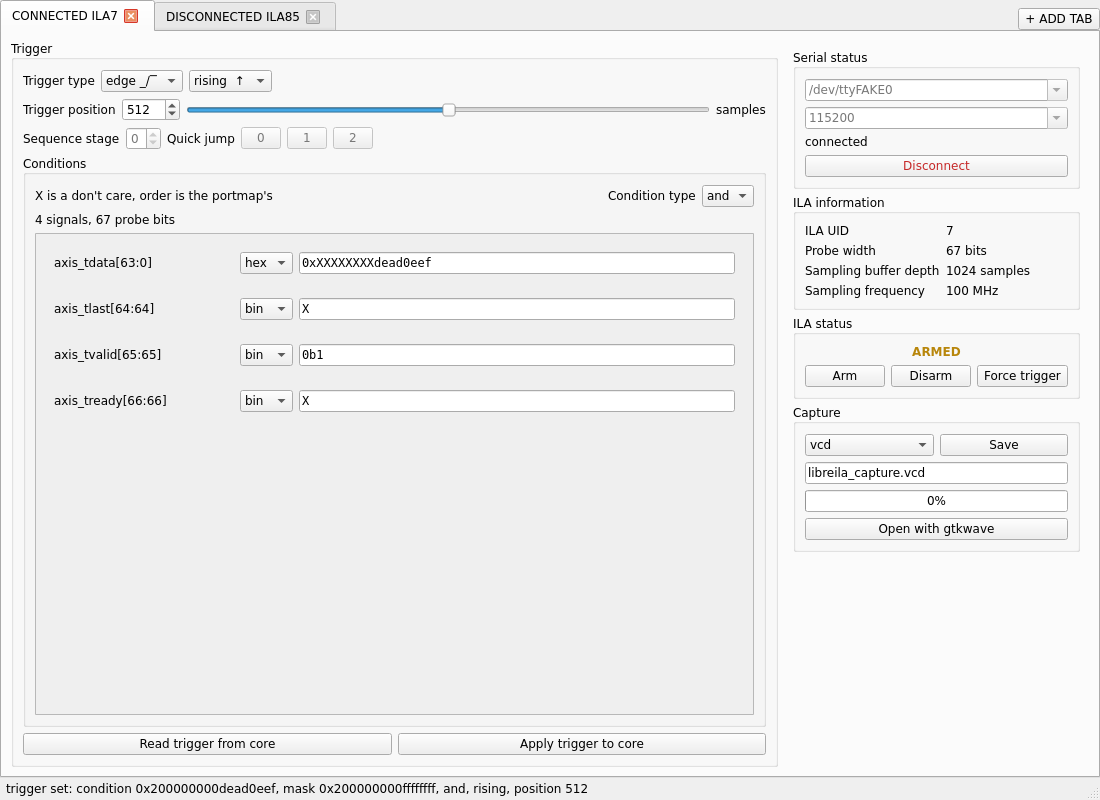
\includegraphics[width=0.8\textwidth]{images/05-armed.png}
    \caption{Image of the GUI showing ILA in armed state.}
    \label{fig:gui-armed}
\end{figure}

\subsection{Watchdog and error handling}
Two safety nets keep a bad link from wedging the wrapper.

A \textbf{watchdog} counts while the wrapper is in any non-idle state
and is cleared whenever a byte makes progress. After
\texttt{G\_AXIL\_CLK\_FREQ} counts, that is one second without progress, the wrapper resets to idle and abandons whatever it had parsed. A timeout therefore loses the whole transaction rather than half applying it, and the host recovers by restarting from its sync byte; since the idle state discards every byte that is not a sync byte, the link resynchronises on its own.

Each request is also \textbf{sanity checked} once its base address is in. The address must be four byte aligned, because the core's decoder truncates rather than rejects and a misaligned write could land on ARM\_FT. The receive \ac{FIFO} is checked for overflow, since the \acs{UART} writes into it unconditionally. A request that fails either check is answered but never put on the AXI bus: a read returns the promised number of zero words, and a write still has its payload drained, so the link stays in step.

\subsection{UART Packet Format}
\label{sec:uartpkt}
The PC is the master of the link. Every transaction is one request packet from the PC and one response packet from the wrapper, both beginning with a sync byte and a six byte header. 

\begin{table}[H]
    \centering
    \begin{tabular}{|l|l|l|}
        \hline
        \rowcolor{gray!40} \textbf{Field} & \textbf{Size} & \textbf{PC to wrapper} \\
        \hline
        SYNC          & 1 byte  & \hex{55} \\
        \hline
        R/W           & 1 bit   & 1 write, 0 read \\
        \hline
        \#words       & 7 bits  & word count, 1 to 127 \\
        \hline
        Base address  & 4 bytes & byte address, 4 byte aligned \\
        \hline
        Write data    & 4 bytes each & \#words words, write only \\
        \hline
    \end{tabular}
    \caption{Request packet}
    \label{tab:reqpkt}
\end{table}

\begin{table}[H]
    \centering
    \begin{tabular}{|l|l|l|}
        \hline
        \rowcolor{gray!40} \textbf{Field} & \textbf{Size} & \textbf{Wrapper to PC} \\
        \hline
        SYNC          & 1 byte  & \hex{AA} \\
        \hline
        valid         & 1 bit   & 1 accepted, 0 refused \\
        \hline
        \#words       & 7 bits  & echoed word count \\
        \hline
        Base address  & 4 bytes & echoed base address \\
        \hline
        Read data     & 4 bytes each & \#words words, read only \\
        \hline
    \end{tabular}
    \caption{Response packet}
    \label{tab:rsppkt}
\end{table}

Points worth knowing about the framing:

\begin{itemize}
    \item Every field wider than a byte goes \textbf{MSB first}, both the base address and the data words. The header is six bytes, the payload $4 \times$ \#words bytes.
    \item The R/W bit and the word count \textbf{share one byte}: bit 7 is R/W, bits 6 downto 0 are the count. The response byte is the same shape, with \emph{valid} in bit 7.
    \item \textbf{One packet moves at most 127 words.} Longer transfers are split across packets with the base address advancing by four per word. This is routine and not an edge case: reading the stock 2048-sample buffer at stride 4 is 8192 words, that is 65 packets.
    \item \textbf{A write is acknowledged too.} The response header goes out as soon as the address has been parsed, before the write data has even arrived, so a host that does not drain the six byte acknowledgement will desynchronise the next transaction. Only a read is followed by data words.
    \item Because the write header precedes the write payload, an overflow during that payload is reported on the \emph{next} packet's header. Overflow detection is best effort: valid = 0 means bytes were dropped, valid = 1 does not promise that none were.
\end{itemize}

\newpage
\section{Additional references}
\begin{itemize}
    \item \textbf{Repository and full documentation} ---
          \url{github.com/yashparitkar/libreila}. This datasheet is the specification for the register map, the trigger vector and the packet format; the repository holds the sources, the drivers, the test suite and the per-directory READMEs covering code generation and driver usage.
    \item \textbf{LibreILA User Manual} --- the full instantiation, generation and debug procedure, of which this datasheet is a summary.
    \item \textbf{License} --- CERN \acf{OHL} Version 2, Permissive. See the \texttt{LICENSE} file in the repository.
    \item \textbf{Microchip G238606} --- PolarFire family fabric user guide, for the \acs{LSRAM} block and its independent read, which the readout path relies on.
    \item \textbf{ARM IHI 0022} --- AMBA \acs{AXI} and ACE protocol specification, for the AXI4Lite slave port.
    \item \textbf{VHDL Style Guide (VSG)} --- recommended for reformatting the generated sources before they are committed to a project.
\end{itemize}

\newpage
\section{Device utilization and performance}
\label{sec:utilization}
Resource usage scales with the two generics that describe the capture, and with nothing else. The storage requirement is exactly

\[
    \mathrm{bits} = \mathtt{G\_SAMP\_BUFF\_DEPTH} \times
                    \mathtt{C\_N\_LANES} \times 32
\]

that is, the probe word rounded up to a whole number of 32-bit lanes. Note that the stride padding used on the bus costs address space only and is not stored, so a 67-bit probe occupies three lanes in RAM and not four. For the stock build that is $2048 \times 3 \times 32 = 196{,}608$ bits, which maps onto PolarFire \acs{LSRAM} blocks.

This design uses UART at 115200 baud and size of both the transmit and receive \acs{FIFO}s is 1024 bytes. The core is clocked at 100 MHz for both clock domains.

\begin{table}[H]
    \centering
    \begin{tabularx}{\textwidth}{|l|l|P|P|P|P|P|P|}
        \hline
        \rowcolor{gray!40} \textbf{Probe width} & \textbf{Depth} & \textbf{Fabric 4LUT} & \textbf{Fabric DFF} & \textbf{Interface 4LUT} & \textbf{Interface DFF} & \textbf{LSRAM (20K)} & \textbf{fmax} \\
        \hline
        67   & 2048 & 1280 & 817 & 360 & 360 & 9 & 243 MHz \\
        \hline
        67 (ext\_trig)  & 2048 & 1015 & 558 & 360 & 360 & 9 & 270 MHz \\
        \hline
        67   & 4096 & 1267 & 828 & 540 & 540 & 14 & 252 MHz \\
        \hline
        35   & 2048 & 1238 & 817 & 288 & 288 & 7 & 252 MHz \\
        \hline
    \end{tabularx}
    \caption{Device utilization, PolarFire SoC. Includes the \acs{UART} wrapper (\acs{UART}, TX/RX \acs{FIFO}s and packet parser) around the \texttt{libre\_ila} core.}
    \label{tab:utilization}
\end{table}

Table~\ref{tab:utilization-core} isolates the \texttt{libre\_ila} core itself, that is the sample buffer, trigger comparator, address decode and AXI4Lite slave state machine, excluding the \acs{UART} wrapper that surrounds it in the \acs{IP} used for this measurement.

\begin{table}[H]
    \centering
    \begin{tabularx}{\textwidth}{|l|l|P|P|P|P|P|}
        \hline
        \rowcolor{gray!40} \textbf{Probe width} & \textbf{Depth} & \textbf{Fabric 4LUT} & \textbf{Fabric DFF} & \textbf{Interface 4LUT} & \textbf{Interface DFF} & \textbf{LSRAM (20K)} \\
        \hline
        67   & 2048 & 600 & 388 & 288 & 288 & 7 \\
        \hline
        67 (ext\_trig)   & 2048 & 352 & 129 & 288 & 288 & 7 \\
        \hline
        67   & 4096 & 595 & 395 & 468 & 468 & 12 \\
        \hline
        35   & 2048 & 556 & 388 & 216 & 216 & 5 \\
        \hline
    \end{tabularx}
    \caption{Device utilization of the \texttt{libre\_ila} core module
        alone, PolarFire SoC.}
    \label{tab:utilization-core}
\end{table}

\end{document}
